\section{Approach}
\label{chap:approach}

As seen in \hyperref[chap:related_work]{section \ref{chap:related_work}}, research proposes various theoretical frameworks and implementations in the area of argumentation mapping. This section introduces the concept of \textit{DialogMap} and gives information about the context and background of the developed prototype (sub-section \ref{sub:dialogmap}), describes general concepts of the implemented prototype (\hyperref[sub:design]{sub-section \ref{sub:design}}) and lay out implementation details (\hyperref[sub:implementation]{sub-section \ref{sub:implementation}}).

\subsection{DialogMap}
\label{sub:dialogmap}


\begin{table*}
\centering
\caption{Requirements for online spatial discussion platforms derived from research presented in sections \ref{subchap:gis_stuff}, \ref{zweivier} and \ref{zweifuenf}}
\label{tab:requirements}
\begin{tabular}{|p{7cm}|p{7cm}|l|} \hline
\textbf{Requirement} & \textbf{Impact} & \textbf{Main Sources}\\ \hline

Explicit spatial references in discussion contributions & Clarify denotation of spatial relationships and make communication more efficient & \cite{Rinner_ArgumentationMaps,Cherubini2007_shared_maps}\\ \hline

Multiple connections to locations and locations created in the context of other contributions in one contribution. & More fine grained references and further clarification. Many-to-many connections possible & \cite{Kessler2005_ArgumentationMapPrototype,Voss2004_Evolution_PGIS,you2009_participatory_map_based,Cai2009_spatial_annotation_deliberation}\\ \hline

Tags and categories alongside discussion contributions can be attached & Support statements of contributions & \cite{Longueville2010_community_based_geoportals_web20,Kessler2005_ArgumentationMapPrototype,Kessler2005_Conflict_Resolution,Tang2005_PPGIS_discussion_forum,zhao2006geodf,you2009_participatory_map_based,Cai2009_spatial_annotation_deliberation}\\ \hline

Two-way highlighting of geo-features and contributions & Visualization of relationships & \cite{Cai2009_spatial_annotation_deliberation,Sidlar2009-AssessmentMapGeocollaborationTool}\\ \hline


Filter and sort contributions by custom rules & Custom overviews, visualization of gaps and thoroughly covered areas & \cite{Voss2004_Evolution_PGIS,you2009_participatory_map_based,Hopfer2007_Communication}\\ \hline

Easy user interface & No impediments for non-technical users. No suppression of participation & \cite{Rinner2009_Web2_argumap,Jankowski2005_community_based_pgis,Tang2005_PPGIS_discussion_forum,zhao2006geodf,you2009_participatory_map_based,Carver2001_PPGIS_Cyberdemocracy}\\ \hline

\end{tabular}
\end{table*}







Following the concept of Rinner's Argumentation Map \cite{Rinner_ArgumentationMaps} and the idea of supporting public deliberation through spatially enhanced dialogs, the concept of \textit{DialogMap} was developed for this thesis. Following the recommendations and suggestions of the research presented in sections \ref{subchap:gis_stuff}, \ref{zweivier} and \ref{zweifuenf}, a set of functional and non-functional requirements were derived. \todo{see Tabel 1?}\\
\textit{DialogMap} is a spatial online discussion platform to support geo-deliberative dialogs performed by citizen initiatives \cite{Cai2009_spatial_annotation_deliberation} \todo{Warum Referenz? Gibt doch noch keine Publikation zu DialogMap oder ;) Was sagt die Referenz hier aus?} . It enables users to make explicit spatial references in their discussion contributions to clarify denotation of spatial relationships. This is achieved by allowing the interlinking of one or multiple words with a location or area on the map of the application \cite{Rinner_ArgumentationMaps}. It is possible to create multiple connections between locations in one contribution, as well as referring to locations created in the context of another contribution to allow more fine grained references. Although recommended by multiple authors, many-to-many connections between locations and words is only possible in very few \cite{Kessler2005_ArgumentationMapPrototype,Voss2004_Evolution_PGIS,you2009_participatory_map_based,Cai2009_spatial_annotation_deliberation} of the implemented systems. It is also possible to create multiple hyperlinks on words or multiple words in the contributions' text. The creation of the references and the text can occur in any order \cite{Voss2004_Evolution_PGIS}. It was found that through allowing explicit spatial references, exchange of information can be made more efficient \cite{Cherubini2007_shared_maps}. \todo{Ich verstehe was Du sagen willst: Du listet die Features von DialogMap auf, mit Verweisen auf verwandte Arbeiten - du kombinierst quasi die besten Features / Empfehlungen von anderen - kannst Du das irgendwo auch nochmal vor der "auflistung" bitte kurz deutlich sagen?}\\
Contributions comprise not only of a text with spatial references and hyperlinks, but is composed of multiple other attributes and properties \cite{Longueville2010_community_based_geoportals_web20,Kessler2005_ArgumentationMapPrototype,Kessler2005_Conflict_Resolution}. Users are able to specify tags and a category and to attach an image to each contribution \cite{Tang2005_PPGIS_discussion_forum,zhao2006geodf,you2009_participatory_map_based,Cai2009_spatial_annotation_deliberation} to support their statements in their contributions. The tags and category of the contribution affect the visual appearance of the geo-features created in its context.\\
\textit{DialogMap} structures contributions chronologically \cite{Cherubini2007_shared_maps,you2009_participatory_map_based}. Contributions can be made without context \todo{was heißt without context?} or as a reply to a contribution. It is possible to edit contributions along with its properties and created references. It \todo{it it} is also possible to mark contributions as deleted, which results in a visual marking of the textual representation as well as the fading of the geo-features created in the context of the contribution \cite{Hopfer2007_Communication}.\\% This further supports the linearity of the structured discussions.\\
Creation of contributions is allowed only after a successful authentication to the system. Users can either register an user account with an e-mail/password combination or authenticate themselves through the third party authentication providers Twitter, Facebook and Google \cite{Sani2011_Scalable_Argumap,chun2014usability}. \todo{Auch wenn Du auf Referenzen verweißt hilfts wenn Du kurz in einem halben Satz sagst warum.}\\
The user interface of \textit{DialogMap} features a map and an area to display the textual representations of a contribution. Spatial and textual representations of the contributions are interlinked by a two way highlighting to indicate the relationships between geo-features and contributions \cite{Cai2009_spatial_annotation_deliberation,Sidlar2009-AssessmentMapGeocollaborationTool}.\\
\textit{DialogMap} allows to filter and search for contributions by categories, tags and by free text. This enables users to create their own contribution overviews \cite{Voss2004_Evolution_PGIS,you2009_participatory_map_based}, and allows users to see gaps and thoroughly covered areas \cite{Hopfer2007_Communication}.\\
The importance of an easy user interface was mentioned by multiple authors \cite{Rinner2009_Web2_argumap,Jankowski2005_community_based_pgis,Tang2005_PPGIS_discussion_forum,zhao2006geodf,you2009_participatory_map_based}. As users are likely non-technical \cite{Cai2009_spatial_annotation_deliberation}, the user interface should not discriminate them, thus suppressing participation \cite{Carver2001_PPGIS_Cyberdemocracy}.\\ %An important technical aspect of the conception and development of an spatial discussion platform is to plan it flexible enough to be reused for multiple use cases \cite{Kessler2005_Conflict_Resolution,Kessler2005_ArgumentationMapPrototype,Sani2011_Scalable_Argumap}. This was adequately honored through the Model-view-controller pattern in both the backend and frontend. Another recommendation was, to make the architecture modular, to make the application scalable \cite{Sani2011_Scalable_Argumap} to serve many users at the same time.
The \textit{DialogMap} concept was developed first and foremost to support public participation on a discussion level. \hyperref[fig:my_ladder]{Figure \ref{fig:my_ladder}} shows the theoretical participation level capabilities of \textit{DialogMap} derived from Arnstein and colleagues \cite{Arnstein1969_citizen_participation,Wiedemann1993355,Connor1988_new_ladder}. \hyperref[tab:requirements]{Table \ref{tab:requirements}} lists the most important requirements along with implications and sources.\\
In order to test the initial idea of supporting public deliberation through spatially enhanced dialogs, a working prototype was developed. The aim was to develop a working prototype, which illustrates the concept of spatially enhanced dialogs. Starting from the concept of \textit{DialogMap}, the implementation of a first prototypical application was started.\todo{Etwas viel wiederholung, working/ first prototype..} The development was done in an iterative and agile approach. The creation of working iterations of the \textit{DialogMap} concept made early feedback possible. The possibility to evaluate the concept in a real world use case with users of scientific citizen initiatives \todo{was ist eine scientific citizen initative? Ev. eher citizen initaitve started by a university group?} presented itself early in the development process. The further development was then conducted with practical advice from members of one scientific citizens' initiative. Their input ranged from general suggestions to opinions of specific features. Thus, the following sections describe the distinct outcome of their input to the developed prototype.

\begin{figure}[!h]
    \centering
    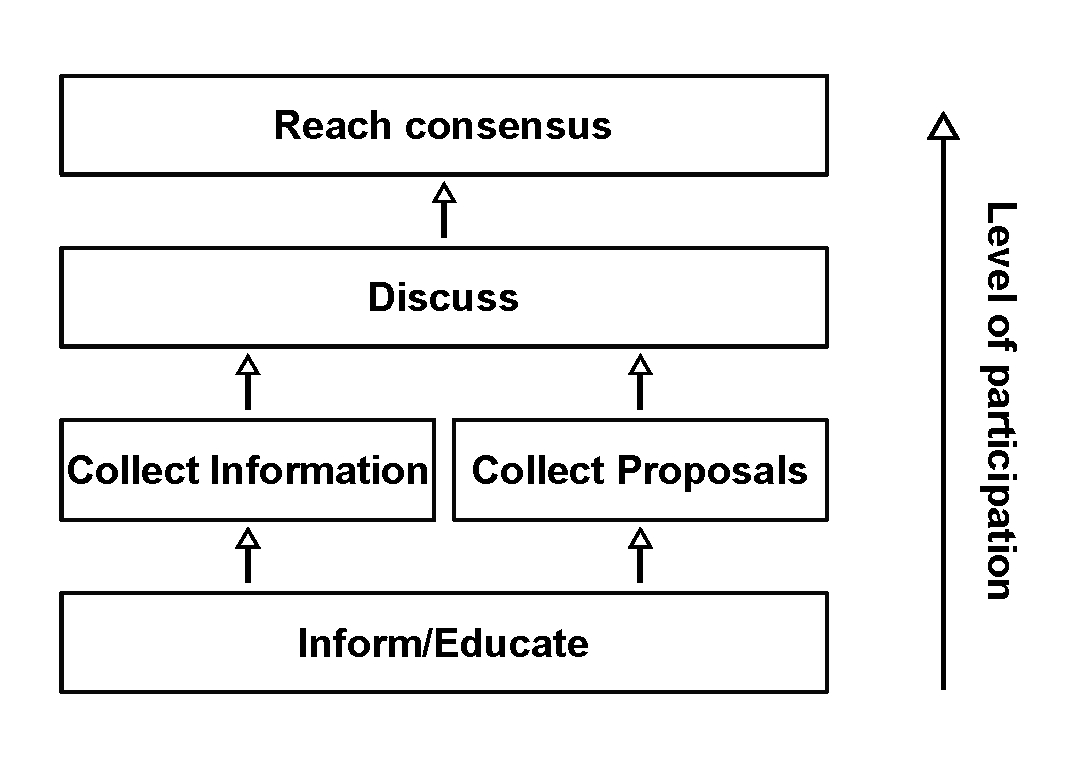
\includegraphics[width=1\columnwidth]{images/my_ladder}
    \caption{Levels of participation of the \textit{DialogMap} concept. Levels adapted from Arnstein and colleagues.}
    \label{fig:my_ladder}
\end{figure}


%``Integrated user interface'', ``Structured discussion'', ``Common (Web)mapping functions'', ``Integrated database, many-to-many relationships'', ``Access control, security'' and ``Customization by Provider''. \cite{Kessler2005_ArgumentationMapPrototype}

%Recommendations for implementing PPGIS \cite{Carver2001_PPGIS_Cyberdemocracy} \cite{Voss2004_Evolution_PGIS}
\todo{Bitte Figure 1 und Tabel 1 stärker im Text erläutern und Ihnen längere captions geben! Die sind gut, und wichtig - aber 3 Stäze pro Ding im Text sollten schon drinn sein!}
\subsection{Application Design} % and features
\label{sub:design}

Internally, the prototype uses few data models. In the configuration used for this thesis, a contribution contains a title, description, two categories, a tags field, a favored counter, an optional time restriction field for start and ending times, an optional image, an optional reference to a parent contribution and optional references to child contributions. The parent and child contribution references create a simple parent-child connection between contributions, as children inherit the categories, tags, time restriction and title. A contribution serves both as a topic and as response to a topic. A contribution also contains references to features, references to feature references and references to URLs.\\
Features are geospatial entities with a location and a reference to its contribution.\\
Feature references contain a title, which can differ from the original title of the feature and a reference to a feature. URL references contain hyperlinks and a description of the hyperlink. The description of a contribution contains the text typed by a user with specially encoded references to features, URL references and feature references. Additionally, each contribution stores the ids of the users who favored it.\\
Users can create contributions in the manner of creating topics or writing responses to existing topics. Users have an e-mail address and a name. \todo{Alles richtige und wichtige Informationen, aber bitte etwas zusammenhängerende Sätze - das ist arg auflistungsartig bis hier. Referenz zu Figure 5 fehlt hier irgendwo?}\\
The front page of the prototype consists of a map with a sidebar. This allows the user to see both spatial and textual representation of contributions at one glance. The right hand sidebar contains the input form for new contributions, filter options, sorting order selector and the list of contributions. The input form consists of input fields for title, categories, time restriction, image and description. The description field allows the creation of spatial features and URL/feature references through connecting words with spatial representations or URLs (See \hyperref[fig:screenshot_create]{Figure \ref{fig:screenshot_create}}). \todo{The. The. The. The.}\\
A text area for arbitrary text and multiple checkboxes allow to restrict the listed contribution as well as the geo-features displayed in the map. It is also possible to change the sorting order of the list of contribution through a drop down field. \hyperref[fig:screenshot_filter]{Figure \ref{fig:screenshot_filter}} depicts the expanded filter with several checkboxes enabled.\todo{Warum wird erst fig 3 referenziert und dann figure 2? Absätze switchen?}

\begin{figure}[!h]
    \centering
    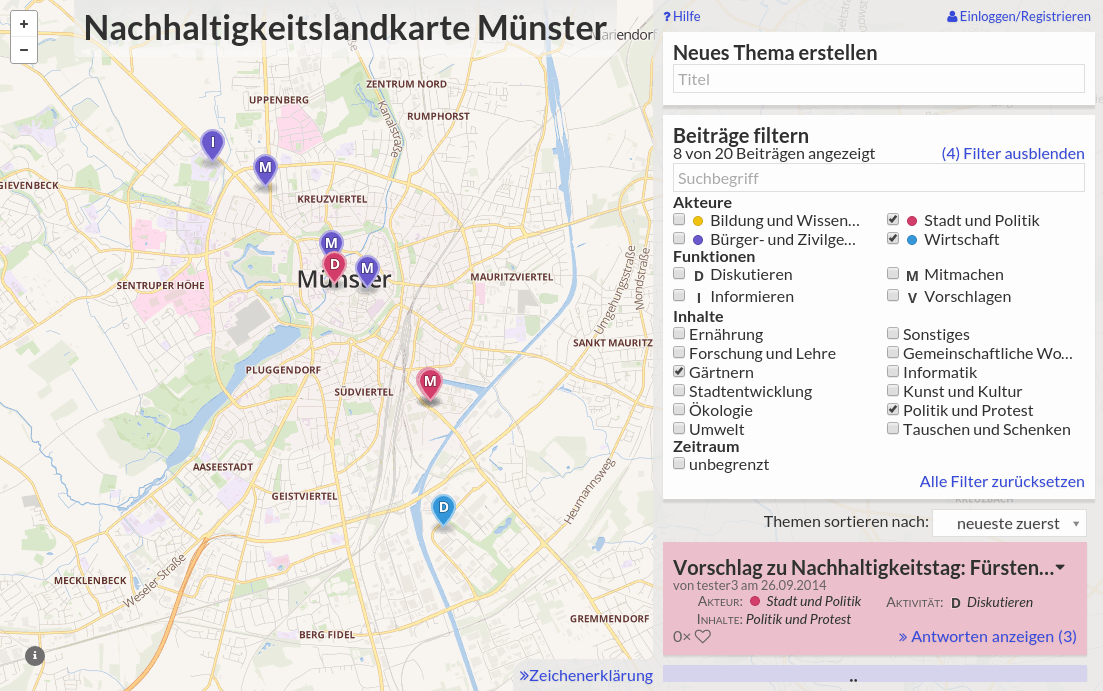
\includegraphics[width=1\columnwidth]{images/screenshot_filters}
    \caption{\textit{DialogMap} with expanded filter in the sidebar. Switching filter options on and off narrows down displayed markers on the map as well as displayed contributions in the sidebar. An input field allows to filter with arbitrary text.}
    \label{fig:screenshot_filter}
\end{figure}

The list of contributions contains colored rectangles representing the different topics. Each rectangle contains the title, time of writing, name of the author, categories, tags and the amount of times the contribution has been favored by users. It also contains a link, which navigates the user to the replies written to the topic. A click on the contribution rectangle expands it vertically, revealing the description of the current topic.\todo{Nicht nur auflisten! Erklären! Verweis auf Bild?}\\
After clicking the ``reply'' link, only the selected topic and replies are shown in the sidebar in a chronological order. In this view, each contribution shows the description by default, as well as author and time and date of writing. The author of the contribution is able to edit and delete the contribution. Upon deletion, the user can enter a reason for deletion, which then will be displayed below the deleted contribution. The deletion is not destructive. The contribution as well as features created for the contribution are marked visually as deleted in order to retain both structure and meaning of the conversation. Other users are able to favor contribution to show interest or agreement.

\begin{figure}[!h]
    \centering
    \includegraphics[width=1\columnwidth]{images/screenshot_create}
    \caption{Input form of \textit{DialogMap} for creating a new topic. Here, all input field are populated by the user. The user has created a spatial reference (green in the lowest box in the sidebar) and a hyperlink (blue box in the lowest box). The color as well as the icon of the marker is determined by the selected categories in the selection fields below the title (``Bürgerbrunch 2014'').}
    \label{fig:screenshot_create}
\end{figure}

The map view contains a base map and several markers and polygons in different colors and different icons in case of markers. These relate to the contributions and are connected through the references in the description of the contributions. Which spatial features are displayed is determined through the state of the sidebar. In the topics overview, only the features created for the starting contributions are displayed in order to prevent cluttering of the view-port. When only a topic and its replies are displayed in the sidebar, all features related to the topic and its replies are shown on the map. \todo{Vielleicht am Anfang dieser Sektion erläutern was eine Contribution ist und was ein Topic? Wies zusammenhängt?}\\
To emphasize the relationship between a contribution and its spatial features, a two way highlighting has been implemented. Hovering over either a contribution-box, marked word or spatial feature on the map triggers visual highlighting on all related contributions, marked words and spatial features. This allows to quickly grasp the relationship between features and contributions. \hyperref[fig:screenshot]{Figure \ref{fig:screenshot}} shows an active highlighting initiated through a mouseover over a marker.\\
Users are able to use either traditional sing-up/sign-in methods or sign-in through different social log-in providers to authenticate to the system.
\todo{Der Abschnitt könnte wirklich gut werden, wenn Du die Bilder etwas stärker referenziert, und Weg vom Auflistungscharakter kommst.. hin zu einem eher flüssig zu lesenden Text. Jetzt ist das eher eine textuelle Featureauflistung. Du bist nah drann das man den Abschnitt gerne list.. und der ist wichtig!}
\begin{figure}[!h]
    \centering
    \includegraphics[width=1\columnwidth]{images/screenshot}
    \caption{Screenshot of the front page of \textit{DialogMap} with active highlight of a contribution and spatial feature. Spatial features are highlighted through a distinct circle. Corresponding contributions are highlighted and scrolled to the top in the sidebar. The highlighting mechanism can be triggered by both pointing on markers and contributions with the mouse pointer.}
    \label{fig:screenshot}
\end{figure}

\subsection{Implementation}
\label{sub:implementation}
\textit{DialogMap} has been implemented from scratch as a single-page web application using AngularJS\footnote{\url{http://angularjs.org/}} and Ruby on Rails\footnote{\url{http://rubyonrails.org/}}. The single-page structure was chosen in order to provide the user with a clear navigation between the overview and contribution answers. This also allows for a seamless browsing experience without full reloads of the page. AngularJS is a JavaScript framework with functionalities like templating, two-way data binding and DOM manipulation. It follows the model-view-controller pattern in order to bring server side paradigms to client-side development. AngularJS was chosen because of its popularity, extensibility and high number of available libraries. It also enables to wrap existing JavaScript libraries to be used in AngularJS context.\\
The mapping library Leaflet\footnote{\url{http://leafletjs.com/}} serves as base for displaying tiled web maps and geospatial data. The user-facing web page was developed using the programming languages CoffeeScript\footnote{\url{http://coffeescript.org/}}, Haml\footnote{\url{http://haml.info/}} and Sass\footnote{\url{http://sass-lang.com/}} to speed up the development. The web page was developed with all major browsers in mind. \todo{The. The. The.}\\
On the server side, components were developed using the Ruby on Rails framework with PostgreSQL\footnote{\url{http://www.postgresql.org/}}/PostGIS\footnote{\url{http://postgis.net/}} as data storage. PostGIS is a spatial database extension for PostgreSQL, which is at the time of writing this thesis, the best option for storing geospatial data. Ruby on Rails, a full-stack model-view-controller web framework, is used as a JSON serving application logic. It was chosen because of its maturity and high number of available libraries. Front- and backend of the prototype communicate in REST-API\footnote{Representational State Transfer Application programming interface} like manner. This allows for easily replaceable front- and backend application stacks.\\
\hyperref[fig:data_structure]{Figure \ref{fig:data_structure}} depicts a generalized data structure diagram.

\begin{figure}[!h]
    \centering
    \includegraphics[width=1\columnwidth]{images/data_structure}
    \caption{Schema of the underlying data structure of the prototype. Time and id fields are omitted for brevity.\todo{Fehlt hier das Topic nicht??}}
    \label{fig:data_structure}
\end{figure}

Every software and libraries used for the development of the prototype are open source. The whole software is open sourced under the Apache License, Version 2.0 \footnote{\url{http://www.apache.org/licenses/LICENSE-2.0}} and is available through GitHub\footnote{\url{https://github.com/ubergesundheit/dialogmap}} for future examination and continuation.


%for styling\footnote{\url{https://github.com/mapbox/simplestyle-spec}}
